\documentclass{report}
\usepackage{amsmath,amssymb,graphicx}
\setlength{\parindent}{0mm}
\setlength{\parskip}{1em}
\begin{document}
\begin{center}

\rule{6in}{1pt} \
{\large
Dongjin Kim
\\ {\bf
$p$-Multigrid for the Nodal Discontinuous Galerkin Approximation
}}


Department of Mathematics \\
University of Wyoming \\
Laramie WY 82071
\\ {\tt
dongkim@uwyo.edu
}
\\
Dan Stanescu
\end{center}



The Discontinuous Galerkin (DG) Method is increasingly used nowadays to
solve advection-dominated problems. Its most attractive features,
namely the high accuracy obtained without the use of an extended
stencil and the inherent parallelization, have turned it into a method
of choice for Computational Fluid Dynamics problems (see the recent
review in [Cockburn,Karniadakis,Shu (2001)]). The early formulation of
the DG method by Cockburn and Shu (1989) uses as degrees of freedom the
coefficients of the solution in a polynomial basis expansion (Legendre
polynomials being used in one dimension to take advantage of their
orthogonality). This modal formulation seems more intuitive, but has a
large drawback for nonlinear problems: to compute nonlinear fluxes, one
needs to first compute the value of the solution by evaluating the
polynomial expansion at the flux integration points, then evaluate the
fluxes. Researchers realized later that this translation from modal
space into physical space can be avoided through a collocation (nodal)
formulation. In the latter framework the degrees of freedom are the
values of the solution at the collocation points, so the flux values
can be evaluated easily, in particular if the collocation points are
chosen to coincide with the integration points
[Stanescu,Hussaini,Farassat (2003)], [Kopriva,Woodruff,Hussaini
(2001)].

In the context of multigrid methods, the modal DG formulation again is
more intuitive: the polynomial-type basis functions can be made
hierarchical, and a $p$-multigrid approach is natural (the restriction
operator for example just neglects extra modes); see recent research in
this direction [Helenbrook,Mavriplis,Atkins (2003)],
[Fidkowski,Darmofal (2003)]. Due to the advantage of the nodal approach
for nonlinear problems, we want to investigate the feasibility of a
$p$-type multigrid method in this latter formulation. It seems that such
an investigation has not been reported yet in the literature. The use
of an acceleration technique such as multigrid may reduce the
difference in cost between the two approaches; however, this is very
likely to be problem dependent, hence arguably a nodal DG $p$-multigrid
method may lead to savings in computer time.

For a preliminary numerical result, we solve the one-dimensional
nonlinear Euler equations and compare the performance (CPU time, MG
cycles) of a nodal DG $p$-multigrid with a modal DG $p$-multigrid.
Figure 1 shows the accuracy versus the number of MG cycles:
\begin{center}
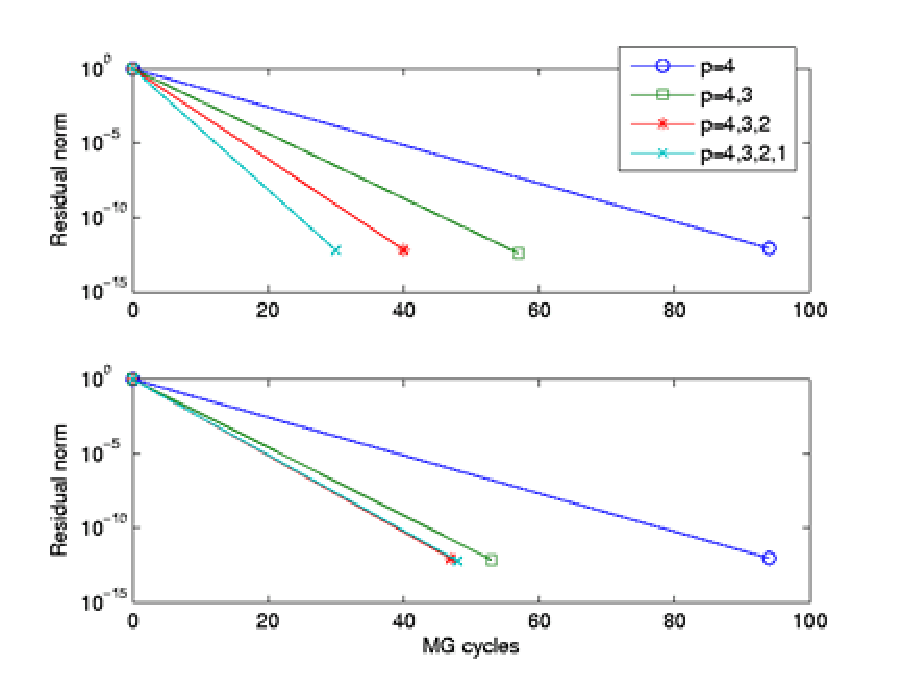
\includegraphics[width=90mm]{KimDfig1}
\end{center}

Figure 2 shows the accuracy versus CPU time:
\begin{center}
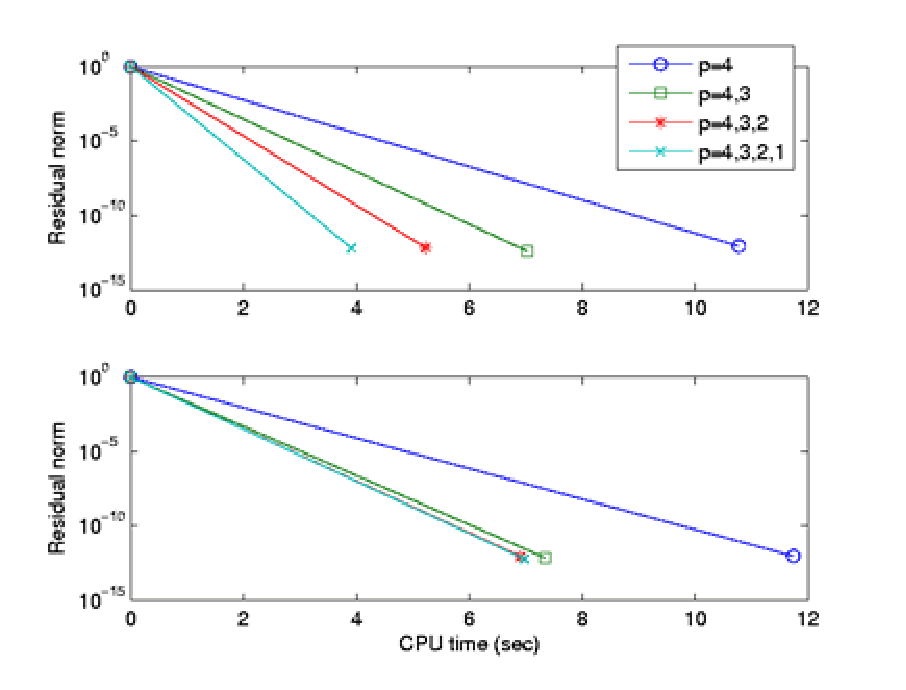
\includegraphics[width=90mm]{KimDfig2}
\end{center}


\end{document}
